\documentclass[10pt,journal,compsoc]{IEEEtran}
\usepackage[brazilian]{babel}
\usepackage[utf8]{inputenc}
\usepackage{graphicx}
\usepackage{minted}
\usepackage{xcolor}
\definecolor{LightGray}{gray}{0.9}
\definecolor{DarkGray}{gray}{0.1}
\usemintedstyle{monokai}


\begin{document}

\title{Filtro Mediana \\ Processamento Paralelo}
\author{André~Thiago~Borghi~Couto,~\IEEEmembership{Graduando,~UFES}
\IEEEcompsocitemizethanks{\IEEEcompsocthanksitem A.T.B. Couto é graduando em ciência da computação, na UFES, campus CEUNES, em São Mateus - ES.\protect\\
E-mail: andreww.max@hotmail.com
}
\thanks{Trabalho escrito em 19 de junho de 2019;}}
\markboth{\LaTeX\ UFES - Processamento Paralelo,~Vol.~1, Mini - EP.~2, Junho~2019}
{Couto \MakeLowercase{\textit{et al.}}: Estudo de paralelização para o filtro de mediana em imagens}

\IEEEtitleabstractindextext{
\begin{abstract}
% Uma demonstração simples do poder computacional, é sem dúvida a edição de imagens, podendo ser aplicada em diversas áreas no nosso mundo, sendo os processos simples ou complexos. Um dos mais básicos que podemos ver em nosso cotidiano é o filtro de mediana, que consiste em reduzir valores que estão muito diferentes de sua vizinhança, obtendo uma imagem mais limpa e nítida.
A simple demonstration of computational power, is undoubtedly the edition of images, being able to be applied in several areas in our world, being the processes simple or complex. One of the most basic we can see in our daily life is the median filter, which consists of reducing values that are very different from your neighborhood, getting a cleaner and sharper image.
\end{abstract}

\begin{IEEEkeywords}
Computer Science, Parallel Programming, \LaTeX, Threads, Ciência da Computação, Pragramação Paralela, OpenMP.
\end{IEEEkeywords}}

\maketitle
\IEEEdisplaynontitleabstractindextext
\IEEEpeerreviewmaketitle
\IEEEraisesectionheading{
    \section{Introdução ao Problema}
        \label{sec:introduction}}

\IEEEPARstart{S}{equancialmente} temos uma complexidade de código em $$O(2^{3nm} + 2^{6n} + 3)$$ diretamente, desconsiderando as chamadas de funções internas, analisando a totalidade do código, temos os seguintes passos:
\begin{itemize}
    \item Leitura da imagem;
    \item Cópia da imagem original;
    \item Cálculo da mediana, (centro da imagem)
    \item Cálculo da mediana, (Bordas da imagem)
    \item Cálculo da mediana, (cantos da imagem)
    \item Gravação da nova imagem;
\end{itemize}

Descrevendo os passos de cálculo de mediana, temos a seleção dos pixel em forma de janela, em volta do pixel analisado, logo obtendo 9 pixels no total, uma função que ordena esses pixels e retorna o pixel central, assim a imagem final tem o filtro aplicado. É relevante saber que as bordas e cantos são separados para evitar falha de segmentação.
Um grande problema identificado nessa implementação é a forma de armazenamento da nova imagem, que a cada execução faz a gravação no disco, e sabemos que utiliza de varias execuções para chegar a um resultado bom, isso interfere diretamente no resultado, por fazer vários acessos no disco. Junto com os acessos a disco, temos o problema da cópia, que torna-se inútil quando estamos trabalhando na produção de uma nova imagem, sem a alteração da anterior.

\section{Estratégia}
Temos identificados os problemas na introdução, agora focamos em otimizá-los.

\subsection{Leitura de disco e Cópia}
Primeiramente procurei a retirada do problema da leitura em disco, com a opção de alocação da memória para a nova imagem:

\begin{minted}[frame=lines, bgcolor=DarkGray, fontsize=\footnotesize, framesep=2mm, baselinestretch=1.2]{c}
    ...
// inde img eh a imagem a ser processada
Imagem *imgDest = (Imagem*)calloc(1,sizeof(Imagem));
imgDest->pixel =aloca(img->altura+2,img->largura+2);
imgDest->altura = img->altura;
imgDest->largura = img->largura;
imgDest->threshold = img->threshold;
    ...
\end{minted}
\label{cod:1}

Juntamente com uma modificação na função, para apenas ser salva ao final das operações, substituindo a função:

\begin{minted}[frame=lines,bgcolor=DarkGray, fontsize=\footnotesize, framesep=2mm, baselinestretch=1.2]{c}
void removeRuidoMediana(char *arqOri,char *arqDes);
\end{minted}

Pelo protótipo:

\begin{minted}[frame=lines,bgcolor=DarkGray, fontsize=\footnotesize, framesep=2mm, baselinestretch=1.2]{c}
Imagem *removeRuidoMediana(Imagem *img);
\end{minted}

Com isso reduzimos um dos loops, após isso o núcleo do código é o próximo passo, onde retiramos loops desnecessários, que são parte do algoritmo original, porém nada otimizado, ao fim podemos colocar todas as instruções de entrada dentro de apenas uma passada por toda a imagem, reduzindo a complexidade do código para $O(3nm)$.

\subsection{Modularização}
A substituição de parte do código por uma função que faz o cálculo da mediana, no caso só encapsulado.

\begin{minted}[frame=lines,bgcolor=DarkGray, fontsize=\footnotesize, framesep=2mm, baselinestretch=1.2]{c}
calcMedia
(int ***im, int imax, int jmax, int k, int mmax){
    int m[9], n = 0;
    for (int i = imax - 1; i <= imax + 1; i++)
        for (int j = jmax - 1; j <= jmax + 1; j++)
            m[n++] = im[i][j][k];
    sort(m, m + mmax);
    return m[mmax / 2];
}
\end{minted}

Comparando as as implementações temos além da redução das linhas de código, a redução do tempo e a legibilidade, em questão de tempo temos um speedup relacionado na tabela %\ref{tab:speedup}

\begin{table}[h]
\label{tab:speedup}
\centering
% \caption{SpeedUp}
\begin{tabular}{r|r|r|r}
Original & Otimizado & 12 Threads & 24 Threads \\
\hline
1,9012      & 1,42  & 1,51  & 1,64 \\
14,79767    & 1,52  & 1,71  & 1,73 \\
11,46187    & 1,58  & 1,68  & 1,70
\end{tabular}
\end{table}

Então podemos considerar que a otimização fez uma grande diferença no desempenho, em média com as modificações que fiz, resultaram em 1.5 em speedup. Continuando com as threads observei a não utilização de 100\% das funções do processador, onde devido a múltiplas trocas simples, os cálculos curtos de média, criaram um gargalo onde cada thread tem um pico de processamento. Assim, a otimização foi considerável, porém a biblioteca Openmp, não nos permite ver especificamente o que está acontecendo, então não tive como nívelar a utilização do poder de processamento.

\section{Testes e Execuções}
Dentre os testes que foram feitos, tive grandes picos de desempenho, e em analises no programa $"top"$, observei por curiosidade uma parte de cada submissão de job, e em todos o $"no"$ estava sendo utilizado por outro processo grande, (como já havíamos visto em um teste da aula), não tenho certeza se interferiu no desempenho dos teste, pois em testes locais no meu pc obtive ganhos próximos, considerando 1, 2, 3 e 4 threads respectivamente.
Podemos ver o gráfico com o resultado do teste final em anexo. %\ref{fig:total}

% \begin{figure}[!ht]
%   \includegraphics[width=0.5\textwidth]{GraficosEP2.png}
%   \caption{Gráfico com todos os testes de desempenho}
%   \label{fig:total}
% \end{figure}

% \newpage
%%%%%%%%%%%%%%%%%%%%%%%%%%%%%%%%%%%%%%%%%%%%%%%%%%%%%%%%%%%%%%%%%%%%%%%%%%%%%%%%%%%%%%
% \appendices
% \section{Gráfico Comparativo Sequencial e Paralelo}
% \begin{figure}[!t]
%   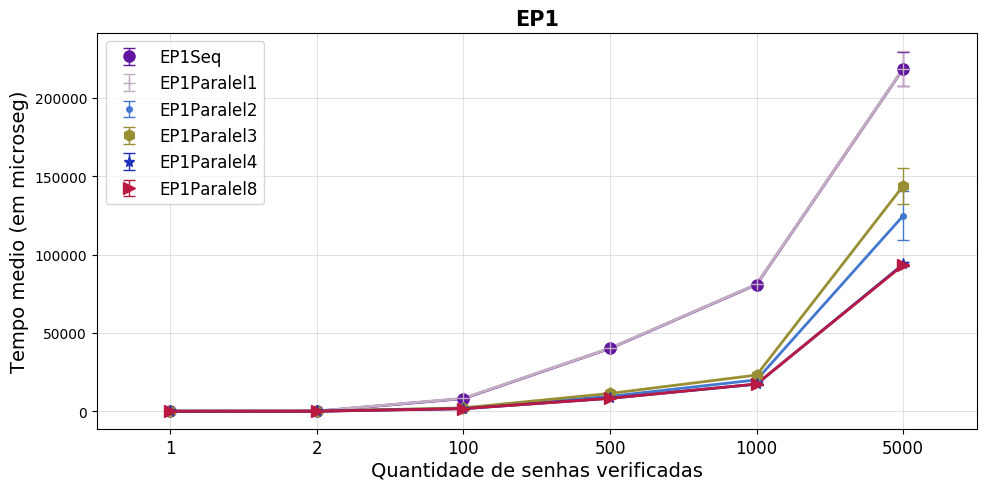
\includegraphics{GraficoEP1-Seq-Par-Nucleo.png}
%   \caption{Gráfico com apenas o tempo do núcleo de busca}
%   \label{figSeqNucleo}
% \end{figure}
% \begin{figure}[!t]
%   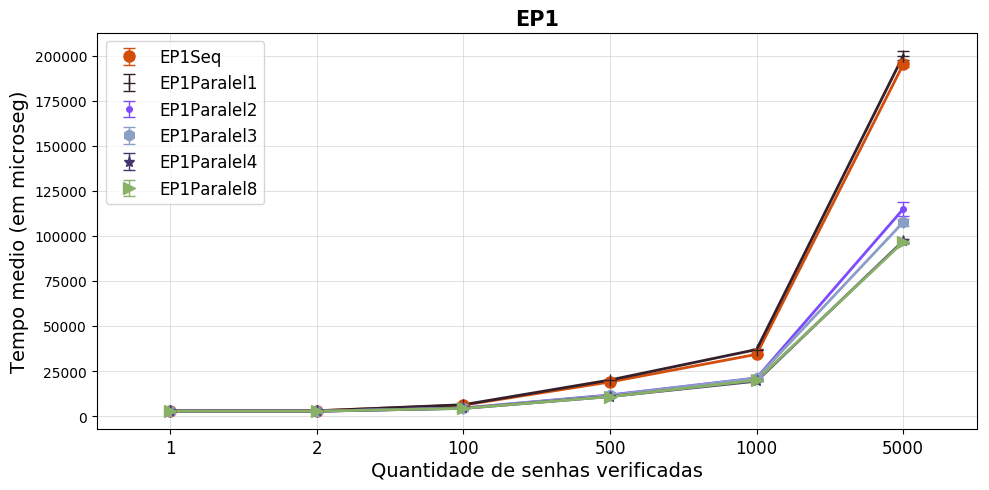
\includegraphics{GraficoEP1-Seq-Par-Total.png}
%   \caption{Gráfico com o tempo do total de execução}
%   \label{figSeqTotal}
% \end{figure}

%%%%%%%%%%%%%%%%%%%%%%%%%%%%%%%%%%%%%%%%%%%%%%%%
% \begin{IEEEbiography}{André Thiago Borghi Couto}
% atualmente cursa graduação em Engenharia da Computação (2016/1) na Universidade Federal do Espírito Santo. Possui conhecimento em desenvolvimento de software, banco de dados, projetos em Arduino, design gráfico e tem interesse nos temas de automação em Arduino, inteligência artificial, redes de computadores e processamento de imagens.
% \end{IEEEbiography}

\begin{IEEEbiographynophoto}{André Thiago Borghi Couto}
atualmente cursa graduação em Engenharia da Computação (2016/1) na Universidade Federal do Espírito Santo. Possui conhecimento em desenvolvimento de software, banco de dados, projetos em Arduino, design gráfico e tem interesse nos temas de automação em Arduino, inteligência artificial, redes de computadores e processamento de imagens.
\end{IEEEbiographynophoto}


\end{document}